\documentclass{article}
\usepackage{tikz, hyperref, comment, amsmath, cleveref, forest, subcaption, listings, xcolor, float}
\usepackage[bottom]{footmisc}
\usepackage[margin=.75in]{geometry}

\renewcommand{\contentsname}{Indice}
\renewcommand{\refname}{Riferimenti}
\renewcommand{\figurename}{Figura}
\renewcommand{\tablename}{Tabella}
\renewcommand{\lstlistingname}{Listato}

\crefformat{section}{\S#2#1#3}
\crefformat{subsection}{\S#2#1#3}
\crefformat{subsubsection}{\S#2#1#3}
\crefformat{figure}{#2Figura~#1#3}
\crefformat{footnote}{#2\footnotemark[#1]#3}
\crefformat{table}{#2Tabella~#1#3}

\crefname{lstlisting}{listato}{listati}
\Crefname{lstlisting}{Listato}{Listati}

\usepackage[listings,skins]{tcolorbox}
\lstdefinelanguage{Toml}{
    comment = [l]{\#},
    keywords = {true, false},
    morestring = [b]{"}
}

\lstset{
    tabsize = 2,
    frame = tb,
    breaklines = true,
    numbers = left,
    numbersep = 5pt,
    numberstyle = \color{white!30!black}\scriptsize,
    stepnumber = 1,
    basicstyle = \footnotesize\ttfamily,
    commentstyle={\color{green!50!black}\ttfamily},
    keywordstyle = {\bfseries\color{purple}}, % keywords
    keywordstyle = [2]{\itshape\color{blue}}, % traits
    keywordstyle = [3]{\color{blue}}, % primitive types
    keywordstyle = [4]{\color{blue}}, % type and value ctors
    keywordstyle = [5]{\color{purple!50!blue}}, % macros
    stringstyle = \color{green!45!blue},
    aboveskip = \baselineskip,
    showstringspaces = false
}
 \lstdefinelanguage{docker}{
  keywords={FROM, RUN, COPY, ADD, ENTRYPOINT, CMD,  ENV, ARG, WORKDIR, EXPOSE, LABEL, USER, VOLUME, STOPSIGNAL, ONBUILD, MAINTAINER, HEALTHCHECK},
  keywordstyle=\color{blue}\bfseries,
  identifierstyle=\color{black},
  sensitive=false,
  comment=[l]{\#},
  commentstyle=\color{purple}\ttfamily,
  stringstyle=\color{red}\ttfamily,
  morestring=[b]',
  morestring=[b]"
}

\title{High performance and quantum computing}

\author{Giuseppe Capasso}

\begin{document}
\begin{titlepage}
  \thispagestyle{empty}
  \raggedright % Allinea a sinistra

  \begin{tikzpicture}
    \node[anchor=south west] at (4,0) {
\includegraphics[scale=0.75]{figures/unina-logo-1.png}};
    \node[anchor=south west] at (0,1.5) {
\includegraphics{figures/unina-logo-2.png}};
    \node[anchor=south west] at (0,0.5) {\textsf{Scuola Politecnica e delle Scienze di Base}};
    \node[anchor=south west] at (0,0) {\textsf{Corso di Laurea Magistrale in Ingegneria Informatica}};
  \end{tikzpicture}

  \vfill

  {\textbf{\textit{\LARGE Tracing e profiling di applicazioni SGX in Linux}}}
  \\[2cm]

  {\textbf{\textit{\Large High Performance and Quantum Computing}}}
  \\[1cm]
  {\large Anno Accademico 2024/2025}

  \vfill

  \begin{table}[h]
    \textbf{Giuseppe Capasso matr. M63001498}
  \end{table}

\end{titlepage}

\thispagestyle{empty}
\tableofcontents

\newpage
\thispagestyle{empty}

\section*{Introduzione}
L'implementazione di Trusted Execution Environment (TEE) in hardware contrasta alcuni \textit{threat model} a discapito delle performance delle applicazioni. Lo scopo di questo progetto è quello di creare un sistema che consenta di raccogliere metriche di applicazioni sia quando vengono eseguite in TEE che non per effettuarne delle comparazioni in futuro. La difficoltà principale nella raccolta metriche in questo tipo di scenari è l'uniformità. Infatti, in TEE hardware, il sistema operativo è visto come non fidato e quindi viene utilizzato in meno possibile dalle applicazioni che potrebbero disabilitare per motivi di sicurezza la raccolta metriche.
L'implementazione proposta si basa su Intel-SGX e utilizza Gramine. Gramine è uno strumento proposto da Intel per effettuare il porting di applicazioni già esistenti in TEE evitando di modificare il codice sorgente.

\clearpage
\section{Requisiti}\label{sec:requirements}
Il sistema che si vuole costruire deve essere in grado di orchestrare l'esecuzione di benchmark di più programmi, eseguendo ogni programma sia con Gramine che senza, variando diverse metriche. I requisiti dell'applicazione sono riassunti nella seguente tabella:

\begin{table}[h]
\centering
\begin{tabular}{|l|p{10cm}|}
\hline
\textbf{Requisito} & \textbf{Descrizione} \\ \hline
R1 & L'applicazione deve essere in grado di eseguire programmi in un ambiente Trusted Execution Environment (TEE) utilizzando Gramine. \\ \hline
R2 & L'applicazione deve eseguire gli stessi programmi anche al di fuori del TEE per consentire il confronto delle prestazioni. \\ \hline
R3 & Deve essere possibile variare le metriche di esecuzione, come il numero di thread, la quantità di memoria allocata, e altre risorse di sistema. \\ \hline
R4 & L'applicazione deve raccogliere metriche di performance durante l'esecuzione dei programmi, sia in TEE che non. \\ \hline
R5 & Deve essere garantita l'uniformità nella raccolta delle metriche, indipendentemente dall'ambiente di esecuzione. \\ \hline
R6 & L'applicazione deve fornire un'interfaccia per configurare e avviare i benchmark in modo automatizzato. \\ \hline
R7 & I risultati dei benchmark devono essere salvati in un formato che consenta un'analisi successiva. \\ \hline
R8 & L'applicazione deve essere in grado di gestire errori e anomalie durante l'esecuzione dei benchmark, fornendo log dettagliati. \\ \hline
R9 & Deve essere possibile eseguire benchmark su diverse piattaforme hardware supportate da Intel-SGX. \\ \hline
\end{tabular}
\caption{Requisiti dell'applicazione per il benchmarking in TEE e non-TEE}
\end{table}

Il benchmark si divide in due tipi principali: Macro benchmark e Micro benchmark. In questa sezione ci concentreremo sui parametri del Macro benchmark, che riguardano l'esecuzione in enclave. I parametri considerati sono i seguenti:

\begin{table}[h]
\centering
\begin{tabular}{|l|p{6cm}|p{6cm}|}
\hline
\textbf{Parametro} & \textbf{Descrizione} & \textbf{Note} \\ \hline
Enclave & Indica se l'esecuzione avviene all'interno di un enclave (Sì/No). & \\ \hline
Memoria Enclave & La quantità di memoria dedicata all'enclave, con valori come "256M". &  A seconda della versione di SGX considerata questo comporterà l'allocazione statica (SGX1) o dinamica (SGX2) della memoria. La memoria EPC ha una grandezza standard che viene configurata dal BIOS e può essere di 64M o 128M  \\ \hline
Numero di thread & Il numero di thread utilizzati dal programma durante l'esecuzione. & A seconda della versione di SGX il numero di thread può crescere staticamente o dinamicamente. Per SGX1, un'enclave ha bisogno di almeno $4$ thread per eseguire (gestore Gramine, servizi di attestazione remota etc.); mentre SGX2 può creare dinamicamente i thread quando c'è bisogno \\ \hline
Tipo di storage & Specifica se lo storage è non fidato (untrusted) o cifrato (encrypted). & \\ \hline
\end{tabular}
\caption{Parametri del Macro benchmark}
\end{table}

Questi parametri sono fondamentali per valutare le prestazioni delle applicazioni quando vengono eseguite in un ambiente Trusted Execution Environment (TEE) utilizzando Gramine. La configurazione di questi parametri consente di analizzare l'impatto delle diverse risorse e configurazioni sull'efficienza e la sicurezza delle applicazioni.

I parametri del micro benchmark sono fondamentali per analizzare il comportamento dettagliato delle applicazioni. I parametri considerati sono i seguenti:

\begin{table}[h]
\centering
\begin{tabular}{|l|p{6cm}|p{6cm}|}
\hline
\textbf{Parametro} & \textbf{Descrizione} & \textbf{Note} \\ \hline
Consumo energetico & Misura l'energia consumata durante l'esecuzione di applicazioni Gramine e non &  \\ \hline
Tracce di esecuzione & Raccoglie le tracce di esecuzione per analizzare il flusso del programma. &  \\ \hline
Pattern di accesso & Analizza i pattern di accesso alla memoria e alle risorse. &  \\ \hline
\end{tabular}
\caption{Parametri del Micro benchmark}
\end{table}

\clearpage
\section{Strumenti per il profiling in Linux}

In questo capitolo si analizzano i principali strumenti messi a disposizione da Linux per il monitoraggio e l'analisi delle prestazioni dei sistemi. In particolare, verranno esaminati i meccanismi basati sui performance counters, le tecniche di misurazione dell'energia e il tracing a livello kernel tramite eBPF.

\subsection{Performance counters}

I performance counters sono strumenti hardware che consentono di monitorare eventi interni alla CPU, come il numero di cicli, cache misses e altri eventi critici per l'analisi delle prestazioni. Linux fornisce l'interfaccia \texttt{perf}\cite{perf-docs}, utilizzabile sia come utility da linea di comando sia in maniera programmatica tramite la system call \texttt{perf\_event\_open}.

La system call \texttt{perf\_event\_open} apre un descrittore di file che rappresenta un contatore di performance. La struttura \texttt{perf\_event\_attr} viene utilizzata per specificare il tipo di evento da monitorare (ad es. cicli CPU, eventi hardware, ecc.), le modalità di raccolta e altre opzioni, come l'esclusione delle attività in kernel o in ambienti virtualizzati.

Di seguito è riportato uno snippet di codice in C che illustra un esempio basilare di utilizzo di \texttt{perf\_event\_open} per monitorare il numero di cicli della CPU:

\begin{lstlisting}[language=C, caption={Esempio di utilizzo di \texttt{perf\_event\_open} per contare i cicli CPU}]
#include <stdio.h>
#include <stdlib.h>
#include <string.h>
#include <unistd.h>
#include <linux/perf_event.h>
#include <sys/ioctl.h>
#include <sys/syscall.h>
#include <asm/unistd.h>
#include <errno.h>

/* Funzione wrapper per la system call perf_event_open */
static long
perf_event_open(struct perf_event_attr *hw_event, pid_t pid, int cpu,
                int group_fd, unsigned long flags) {
    return syscall(__NR_perf_event_open, hw_event, pid, cpu, group_fd, flags);
}

int main(void) {
    struct perf_event_attr pe;
    long fd;
    long long count;

    /* Inizializza la struttura a zero e configura l'evento da monitorare */
    memset(&pe, 0, sizeof(struct perf_event_attr));
    pe.type = PERF_TYPE_HARDWARE;
    pe.size = sizeof(struct perf_event_attr);
    pe.config = PERF_COUNT_HW_CPU_CYCLES;
    pe.disabled = 1;
    pe.exclude_kernel = 1;
    pe.exclude_hv = 1;

    /* Apre il contatore per il processo corrente su tutti i core (-1) */
    fd = perf_event_open(&pe, 0, -1, -1, 0);
    if (fd == -1) {
        perror("perf_event_open");
        exit(EXIT_FAILURE);
    }

    ioctl(fd, PERF_EVENT_IOC_RESET, 0);
    ioctl(fd, PERF_EVENT_IOC_ENABLE, 0);

    /* Inserire qui il lavoro da monitorare */
    sleep(1);

    ioctl(fd, PERF_EVENT_IOC_DISABLE, 0);
    read(fd, &count, sizeof(long long));
    printf("CPU cycles: %lld\n", count);

    close(fd);
    return 0;
}
\end{lstlisting}

In questo esempio, la struttura \texttt{perf\_event\_attr} viene configurata per contare i cicli CPU (\texttt{PERF\_COUNT\_HW\_CPU\_CYCLES}) escludendo il codice kernel e le operazioni in ambienti virtualizzati. Dopo aver aperto il contatore tramite \texttt{perf\_event\_open}, il contatore viene resettato, abilitato, e successivamente disabilitato per leggere il valore accumulato, che viene stampato a video.

\subsection{Misurazione dell'energia}
La tecnologia \emph{Running Average Power Limit (RAPL)}\cite{rapl-docs} consente di monitorare il consumo energetico del sistema suddividendolo in in domini di potenza, quali \textit{package}, \textit{core}, \textit{uncore} e \textit{DRAM},  sfruttando contatori hardware che vengono incrementati in base alla corrente e alla tensione misurate. Questi contatori forniscono una stima dell'energia consumata, espressa in microjoule, e sono esposti dal kernel Linux tramite il filesystem \texttt{sysfs}.

\paragraph{Interfaccia Sysfs}

L'interfaccia RAPL è accessibile in Linux all'interno della directory:

\begin{forest}
for tree={
    font=\ttfamily,
    grow'=0,
    child anchor=west,
    parent anchor=south,
    anchor=west,
    calign=first,
    edge path={
      \noexpand\path [draw, \forestoption{edge}]
      (!u.south west) +(7.5pt,0) |- node[fill,inner sep=1.25pt] {} (.child anchor)\forestoption{edge label};
    },
    before typesetting nodes={
      if n=1
        {insert before={[,phantom]}}
        {}
    },
    fit=band,
    before computing xy={l=15pt},
  }
  [/sys/devices/virtual/powercap
          [intel-rapl
            [enabled]
            [intel-rapl:i
              [enabled]
              [energy\_uj]
              [max\_energy\_range\_uj]
              [name]
              [intel-rapl:i:j
                [enabled]
                [energy\_uj]
                [max\_energy\_range\_uj]
                [name]
              ]
            ]
          ]
        ]
      ]
    ]
  ]
\end{forest}

In questa struttura, l'indice \texttt{i} rappresenta il dominio energetico principale (ad esempio, un package CPU) e l'indice \texttt{j} identifica eventuali sotto-domini (ad esempio, i core interni o la DRAM). Il file \texttt{energy\_uj} contiene il valore cumulativo dell'energia consumata in microjoule, mentre \texttt{max\_energy\_range\_uj} specifica il massimo valore raggiungibile prima che il contatore si resetti.

\paragraph{Implementazione e limiti di RAPL}

I contatori RAPL sono implementati direttamente in hardware:  
\begin{itemize}
    \item \textbf{Misurazione hardware:} Il consumo energetico viene stimato in base alla corrente e alla tensione rilevate da sensori integrati, aggiornando continuamente i contatori.
    \item \textbf{Modelli interni:} I valori riportati sono basati su modelli interni del processore, il che può comportare una certa discrepanza rispetto al consumo reale, soprattutto in condizioni di carico variabile.
    \item \textbf{Risoluzione e wrap-around:} La risoluzione tipica in microjoule potrebbe non essere sufficiente per analisi ad altissima frequenza, e, essendo contatori cumulativi, se non letti con sufficiente frequenza, possono raggiungere il loro limite massimo e conseguentemente "wrap-around", rendendo necessaria una gestione attenta per evitare errori di interpretazione.
\end{itemize}

\subsubsection{Consumo energetico di un disco}
Lo standard RAPL è stato proposto da Intel e implementato anche su alcuni processori AMD. Tuttavia, non esiste uno standard per misurare il consumo energetico di un disco, ma possono essere ottenute delle metriche indirette a partire dal numero di byte scritti, conoscendo la configurazione di base del sistema e le specifiche del disco utilizzate.

Ad esempio, assumendo di avere un disco rotazionale con 7200rpm, il consumo energetico può variare in base al tipo di operazione di scrittura. Supponiamo che il consumo medio per una scrittura sequenziale di 1GB sia di circa 5W, mentre per una scrittura casuale sia di circa 10W, a causa del maggiore movimento delle testine. Se ipotizziamo di scrivere un totale di \(x\) byte, di cui il 70\% in modalità sequenziale e il 30\% in modalità casuale, il consumo energetico totale può essere stimato come segue:

\begin{itemize}
  \item Consumo per scrittura sequenziale: \(0.7 \times \frac{x}{1 \text{GB}} \times 5 \text{W}\);
  \item Consumo per scrittura casuale: \(0.3 \times \frac{x}{1 \text{GB}} \times 10 \text{W}\)
\end{itemize}

I dischi SSD (e nvme) non risentono della differenza di operazioni sequenziali e randomiche.

\subsection{Tracing a livello kernel: eBPF}
\emph{extended Berkeley Packet Filter (eBPF)}\cite{ebpf-docs} è una tecnologia utilizzata per eseguire programmi all'interno del kernel senza scrivere moduli kernel. Il vantaggio di questa scelta risiede nel fatto che l'ambiente in cui eseguono questi programmi è isolato e, pertanto, un \textit{crash} del programma non impatta il fallimento del kernel.

Un programma eBPF è composto da diverse sezioni, tra cui le sezioni `.maps`, che definiscono le strutture dati utilizzate per memorizzare le informazioni raccolte durante l'esecuzione. Queste mappe sono essenziali per trasferire i dati dal kernel allo spazio utente. Un aspetto distintivo dei programmi eBPF è che non hanno un punto di ingresso `main` come i programmi tradizionali. Invece, vengono attaccati (attraverso la primitiva \textbf{\textit{attach}}) a specifici eventi o punti di hook nel kernel, come l'entrata o l'uscita da una system call.

\subsubsection{Architettura eBPF}
eBPF è una macchina virtuale (simile alla JVM) instanziata all'interno del kernel per l'esecuzione di funzioni in \textit{kernel-space}. La macchina è di tipo RISC e ha $11$ registri a $64-bit$, uno stack limitato a $512$ byte. Questa macchina effettua dei salti alle istruzioni da eseguire utilizzando una coda dei programmi.

Questa macchina è dotata di un JIT (Just in time compiler) che consente di compilare in codice macchina il codice oggetto passato in ingresso, generate con un compilatore \textit{LLVM-compliant}. Come mostrato in \cref{fig:ebpf_arch}, prima di essere caricato in memoria, il programma passa per un \textit{verifier}. Questo applica delle regole per capire se:
\begin{itemize}
  \item il programma effettua cicli infiniti;
  \item accede ad aree di memoria illecite e/o non inizializzate
\end{itemize}

\begin{figure}
  \begin{center}
    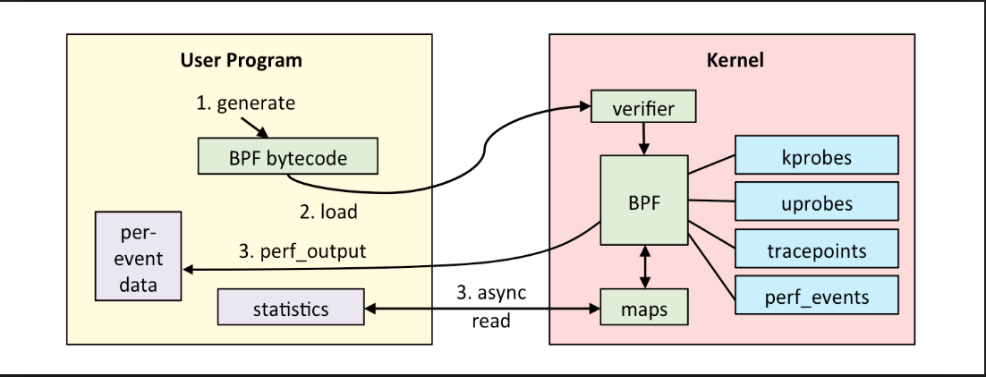
\includegraphics[width=0.95\textwidth]{./figures/ch2/ebpf_arch.png}
  \end{center}
  \caption{Flusso di un programma eBPF}\label{fig:ebpf_arch}
\end{figure}


\paragraph{Struttura di un programma eBPF} Di seguito è riportato un programma eBPF che invia in spazio utente ogni volta che viene chiamata la system call \texttt{read}. Il programma dichiara un ringbuffer a cui si dovrà sottoscrivere il programma user-space per ottenere gli eventi.
\begin{lstlisting}[language=C, caption={Esempio di un programma eBPF che invia in user-space tutte le operazioni sys\_enter\_read}]
#include <linux/bpf.h>
#include <bpf/bpf_helpers.h>

#define EVENT_SYS_READ 0

struct event {
  __u32 ev_type;
  __u64 timestamp;
};

struct {
  __uint(type, BPF_MAP_TYPE_RINGBUF);
  __uint(max_entries, 1 << 20);
} events SEC(".maps");

static __always_inline int snd_trace_event(__u32 evt) {
  __u64 ts = bpf_ktime_get_ns();
  struct event *rb_event = bpf_ringbuf_reserve(&events, sizeof(struct event), 0);

  if (!rb_event) {
    bpf_printk("bpf_ringbuf_reserve failed\n");
    return 1;
  }

  rb_event->ev_type = evt;
  rb_event->timestamp = ts;

  bpf_ringbuf_submit(rb_event, 0);

  return 0;
}

SEC("tracepoint/syscalls/sys_enter_read")
int trace_enter_read(struct trace_event_raw_sys_enter *ctx) {
  return snd_trace_event(EVENT_SYS_READ); 
}

char LICENSE[] SEC("license") = "GPL";
\end{lstlisting}

Questo programma può essere compilato in $2$ fasi. Il primo comando genera una rappresentazione intermedia del programma ($IR$), mentre il secondo lo converte in codice oggetto.
\begin{verbatim}
clang -S -g -target bpf -Wall -Werror -O2 -o prog.ll -emit-llvm -c prog.bpf.c 
llc -march=bpf -filetype=obj -O2 -o prog.o prog.ll
\end{verbatim}

Il codice oggetto può essere caricato nel kernel attraverso \textit{bpftool} da cui si può ottenere un disassmblato dopo la fase di compilazione e verifica.

\begin{verbatim}
sudo bpftool prog load prog.o /sys/fs/bpf/prog
sudo bpftool prog dump jited name dump_bpf_prog
\end{verbatim}

Il programma di seguito carica quello ebpf e stampa tutti gli eventi ricevuti dal ringbuffer.

\begin{lstlisting}[language=C, caption={Esempio di un programma user-space che riceve gli eventi dal ringbuffer}]
#include <stdio.h>
#include <stdlib.h>
#include <signal.h>
#include <bpf/libbpf.h>
#include <bpf/bpf.h>

static volatile int stop;

struct event {
  __u32 ev_type;
  __u64 timestamp;
};

void handle_signal(int signo) { stop = 1; }

int handle_event(void *ctx, void *data, unsigned long ata_sz) {
  struct event *e = (struct event *)data;
  printf("Evento ricevuto: tipo=%u, timestamp=%llu ns\n", e->ev_type,
         e->timestamp);
  return 0;
}

int main() {
  struct ring_buffer *rb = NULL;
  struct bpf_link *link = NULL;
  struct bpf_program *prog;
  struct bpf_object *obj;
  int err;

  obj = bpf_object__open_file("prog.o", NULL);
  if (!obj) {
    fprintf(stderr, "Errore nel caricamento del programma eBPF\n");
    return 1;
  }

  err = bpf_object__load(obj);
  if (err) {
    fprintf(stderr, "Errore nel caricamento dell'oggetto BPF: %d\n", err);
    goto cleanup;
  }

  prog = bpf_object__find_program_by_name(obj, "trace_enter_read");
  if (!prog) {
    fprintf(stderr, "Errore nel trovare il programma BPF\n");
    goto cleanup;
  }

  link = bpf_program__attach_tracepoint(prog, "syscalls", "sys_enter_read");
  if (!link) {
    fprintf(stderr, "Errore nell'aggancio del programma eBPF\n");
    goto cleanup;
  }

  signal(SIGINT, handle_signal);
  signal(SIGTERM, handle_signal);

  rb =
      ring_buffer__new(bpf_map__fd(bpf_object__find_map_by_name(obj, "events")),
                       handle_event, NULL, NULL);
  if (!rb) {
    fprintf(stderr, "Errore nell'apertura della ring buffer\n");
    goto cleanup;
  }

  printf("In ascolto degli eventi... (Ctrl+C per terminare)\n");

  while (!stop) {
    err = ring_buffer__poll(rb, 100); // Poll con timeout di 100ms
    if (err < 0) {
      fprintf(stderr, "Errore nella ring buffer poll: %d\n", err);
      break;
    }
  }

  printf("\nTerminazione...\n");

cleanup:
  ring_buffer__free(rb);
  bpf_link__destroy(link);
  bpf_object__close(obj);
  return 0;
}
\end{lstlisting}

Il \textit{main} può essere compilato linkando la libreria bpf (che deve essere installata):

\begin{verbatim}
gcc -o user-space -lbpf main.c
\end{verbatim}

\clearpage
\section{Implementazione}
Il sistema descritto in \cref{sec:requirements} è implementato in un'applicazione CLI in Rust. Il progetto si trova in \cite{eb-repo}, mentre la documentazione è disponibile in \cite{eb-docs}.
\subsection{Architettura}
L'architettura dell'applicazione è mostrata in \cref{fig:eb_cli_arch}. Il sistema utilizza diversi thread, ognuno dei quali si occupa di raccogliere metriche specifiche durante l'esecuzione del programma. In particolare, l'applicazione si avvale di:
\begin{itemize}
  \item \textbf{eBPF collector}: un modulo che sfrutta eBPF per attaccare dei programmi al kernel, in modo da tracciare eventi a basso livello come le chiamate di sistema (ad esempio, \texttt{sys\_enter\_read}) e operazioni I/O. Questi dati vengono poi memorizzati in apposite strutture dati (mappe) e salvati in file CSV.
  \item \textbf{Energy monitor}: un thread dedicato che, mediante la tecnologia RAPL, esegue il polling dei contatori energetici disponibili nel kernel. Il monitoraggio viene effettuato leggendo i file relativi ai domini di potenza (ad es. \texttt{intel-rapl:0}, \texttt{intel-rapl:0:0}, ecc.) e salvando i dati con timestamp e consumo in microjoule.
  \item \textbf{Performance counters}: un processo esterno viene lanciato per sfruttare l'interfaccia \textit{perf} del kernel, consentendo la raccolta di contatori hardware e altri eventi di performance. I dati vengono raccolti in un file \texttt{perf.csv}.
\end{itemize}

\begin{figure}
  \begin{center}
    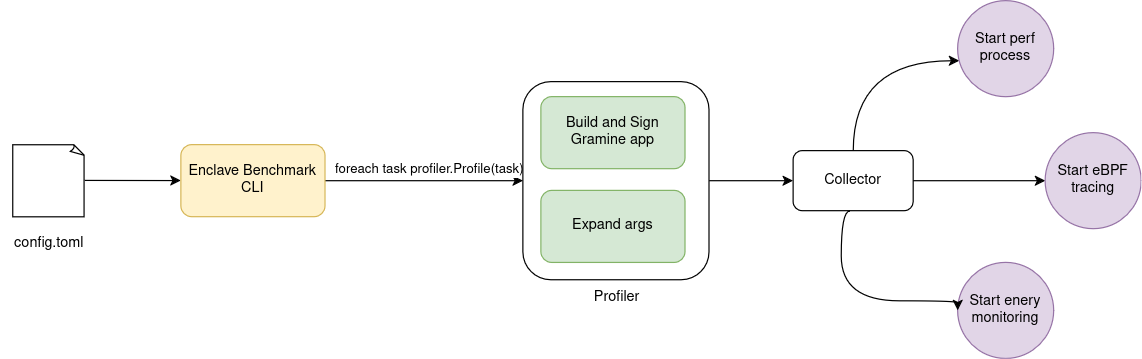
\includegraphics[width=0.95\textwidth]{./figures/ch3/eb_cli_arch.png}
  \end{center}
  \caption{Struttura generale dell'applicazione}\label{fig:eb_cli_arch.png}
\end{figure}

Gli esperimenti sono generati dinamicamente in base alla combinazione di parametri definiti nel file di configurazione, quali il numero di thread (\texttt{globals.num\_threads}), la dimensione dell'enclave (\texttt{globals.enclave\_size}) e, per le applicazioni basate su Gramine, il tipo di storage (\texttt{task.storage}). Ad ogni esperimento corrisponde una specifica directory contenente, oltre ai dati raccolti, il manifesto e la firma dell'enclave (per Gramine), e le directory per i file cifrati e non cifrati.

\subsection{Installazione}
Questa sezione illustra in dettaglio come preparare l'host e installare l'applicazione. Poiché Rust è supportato su tutte le principali piattaforme e sistemi operativi, il vincolo principale riguarda Gramine. Infatti, essendo Gramine costruito da sorgente (necessario per il profiling delle applicazioni) e supportato su ogni sistema compatibile con la piattaforma SGX, è fondamentale che il driver SGX sia incluso nel kernel. A partire dalla versione 5.11 del kernel Linux (con la configurazione \texttt{CONFIG\_X86\_SGX=y}), il supporto è abilitato di default.

\subsubsection{Host Setup}
Per preparare l'host esistono tre possibili approcci:

\begin{itemize}
  \item \textbf{Utilizzo di uno script:} Per Ubuntu 22.04 e 24.04 è disponibile uno script rapido (\texttt{dev/setup\_host.sh}) che configura automaticamente l'ambiente. Per eseguirlo, lanciare:
  \begin{verbatim}
sudo ./dev/setup_host.sh
  \end{verbatim}

  \item \textbf{Installazione su bare metal:} Se si preferisce installare manualmente le dipendenze su Ubuntu 24.04, seguire i passaggi descritti di seguito.

  \item \textbf{Creazione di un'immagine Docker:} È possibile creare un container Docker che includa l'ambiente di build, utile soprattutto se non si utilizza Ubuntu 24.04.
\end{itemize}

\paragraph{Bare Metal}
Per una configurazione manuale su Ubuntu 24.04, procedere come segue:

\begin{enumerate}
  \item \textbf{Abilitare SGX in BIOS:} Assicurarsi che la tecnologia Intel SGX sia abilitata nelle impostazioni del BIOS.

  \item \textbf{Installare le dipendenze di build:} Queste dipendenze sono necessarie per compilare sia Gramine da sorgente che l'applicazione di benchmark. Eseguire:
  \begin{verbatim}
sudo apt-get install -y build-essential clang clang llvm-dev python3-dev \
libbpf-dev git autoconf bison gawk meson nasm pkg-config python3 python3-click \
python3-jinja2 python3-pyelftools python3-tomli python3-tomli-w python3-voluptuous \
wget cmake libprotobuf-c-dev protobuf-c-compiler protobuf-compiler python3-cryptography \
python3-pip python3-protobuf curl linux-tools-$(uname -r)
  \end{verbatim}

  \item \textbf{Installare il software SGX:} Aggiungere il repository e installare i pacchetti necessari:
  \begin{verbatim}
echo 'deb [signed-by=/etc/apt/keyrings/intel-sgx-keyring.asc arch=amd64] 
https://download.01.org/intel-sgx/sgx_repo/ubuntu noble main' | \
sudo tee /etc/apt/sources.list.d/intel-sgx.list
wget https://download.01.org/intel-sgx/sgx_repo/ubuntu/intel-sgx-deb.key
cat intel-sgx-deb.key | sudo tee /etc/apt/keyrings/intel-sgx-keyring.asc > /dev/null
sudo apt-get update
sudo apt-get install libsgx-dcap-quote-verify-dev libsgx-epid libsgx-quote-ex libsgx-dcap-ql
  \end{verbatim}

  \item \textbf{Installare la toolchain Rust:} Utilizzare \texttt{rustup} per installare Rust:
  \begin{verbatim}
curl --proto '=https' --tlsv1.2 -sSf https://sh.rustup.rs | sh
  \end{verbatim}
\end{enumerate}

\subsubsection{Building di Gramine}
Per compilare Gramine (versione 1.8) da sorgente, seguire questi passaggi:

\begin{enumerate}
  \item \textbf{Recuperare il codice sorgente:}
  \begin{verbatim}
git clone --depth=1 --branch v1.8 https://github.com/gramineproject/gramine.git
cd gramine
git checkout v1.8
  \end{verbatim}

  \item \textbf{Configurare, compilare e installare Gramine:} Utilizzare \texttt{meson} per la configurazione e la compilazione. È importante impostare il parametro \texttt{buildtype} a \texttt{debugoptimized} (oppure \texttt{debug}) per abilitare il profiling delle applicazioni Gramine. Se si desidera utilizzare \texttt{musl} come libc, passare l'argomento \texttt{-Dlibc=musl}.
  \begin{verbatim}
meson setup build/ --buildtype=debugoptimized -Dsgx=enabled -Ddcap=enabled -Dlibc=glibc
meson compile -C build/
sudo meson compile -C build/ install
  \end{verbatim}
\end{enumerate}

\subsubsection{Creazione di un Container Docker}
Se non si utilizza Ubuntu 24.04, è possibile creare un'immagine Docker utilizzando il file \texttt{dev/Dockerfile}. Per costruire l'immagine, eseguire:
\begin{verbatim}
docker build -t enclave-benchmark-dev - <dev/Dockerfile
\end{verbatim}
Il processo di build può richiedere tempo, poiché compila \texttt{perf} e \texttt{libbpf} a partire dal codice sorgente del kernel host. Per avviare un container Docker (assicurarsi di utilizzare l'opzione \texttt{--privileged} per accedere ai contatori di performance) e mappare il dispositivo SGX (\texttt{/dev/sgx\_enclave}), utilizzare:
\begin{verbatim}
docker run -it -w /app -v $(pwd):/app --privileged --device /dev/sgx_enclave\
--name enclave-benchmark enclave-benchmark-dev
\end{verbatim}

\subsubsection{Compilazione dell'applicazione da sorgente}
L'applicazione è attualmente installabile \textbf{solo} compilando il codice sorgente, in quanto dipende fortemente dal sistema operativo host. Per compilare l'applicazione:

\begin{enumerate}
  \item \textbf{Clonare la repository:}
  \begin{verbatim}
git clone https://github.com/alarmfox/enclave-benchmark.git
  \end{verbatim}

  \item \textbf{Installare il toolchain Rust:} Installare Rust tramite \url{https://rustup.rs/} seguendo le istruzioni fornite.

  \item \textbf{Generare il file \texttt{vmlinux.h}:} Questo file è necessario per compilare i programmi eBPF. Eseguire:
  \begin{verbatim}
bpftool btf dump file /sys/kernel/btf/vmlinux format c > src/bpf/vmlinux.h
  \end{verbatim}

  \item \textbf{Compilare l'applicazione:} Per una build ottimizzata, eseguire:
  \begin{verbatim}
cargo build --release
  \end{verbatim}
  (Rimuovere il flag \texttt{--release} per una compilazione più rapida ma non ottimizzata.)

  \item \textbf{(Opzionale) Copiare l'eseguibile:} Se necessario, è possibile copiare l'eseguibile in una posizione a scelta:
  \begin{verbatim}
cp target/<debug|release>/enclave-benchmark .
  \end{verbatim}

  \item \textbf{Eseguire l'applicazione:} Verificare l'installazione eseguendo:
  \begin{verbatim}
./enclave-benchmark -V
  \end{verbatim}
  L'output atteso dovrebbe essere simile a:
  \begin{verbatim}
enclave-benchmark 0.1.0
  \end{verbatim}
\end{enumerate}

\subsection{Utilizzo}
L'applicazione richiede un file di configurazione in formato \texttt{TOML} per eseguire una serie di benchmark in sequenza. I file di esempio si trovano nella directory \texttt{examples}. Ad esempio, il file \texttt{examples/full.toml} è strutturato come segue:

\begin{verbatim}
[globals]
sample_size = 3
enclave_size = ["64M", "128M"]
output_directory = "/tmp/test"
num_threads = [1, 2]
extra_perf_events = ["cpu-clock"]
energy_sample_interval = "250ms"
debug = true

[[tasks]]
executable = "/bin/dd"
args = ["if=/dev/zero", "of=/dev/null", "count=10000"]

[[tasks]]
pre_run_executable = "/usr/bin/echo"
pre_run_args = ["Starting make"]

executable = "/usr/bin/make"
args = ["-C", "examples/basic-c-app/", "-j", "{{ num_threads }}", "app", "output={{ output_directory }}"]

post_run_executable = "/usr/bin/make"
post_run_args = ["-C", "examples/basic-c-app", "clean", "output={{ output_directory }}"]

[[tasks]]
executable = "examples/simple-writer/writer"
args = ["{{ output_directory }}"]
storage_type = ["encrypted", "tmpfs", "untrusted"]
\end{verbatim}

\subsubsection*{Specifiche del File di Input}
Il file di configurazione \texttt{TOML} è organizzato in due sezioni principali: \texttt{[globals]} e \texttt{[[tasks]]}.

\paragraph{Configurazione Globale (\texttt{[globals]})}
Questa sezione definisce le impostazioni che si applicano a tutte le esecuzioni dei benchmark:
\begin{itemize}
  \item \textbf{sample\_size} (integer): specifica il numero di ripetizioni per ogni esperimento.
  \item \textbf{enclave\_size} (lista di stringhe): definisce le diverse dimensioni della memoria per l'enclave (es. \texttt{"64M"} e \texttt{"128M"}).
  \item \textbf{output\_directory} (stringa): directory in cui vengono salvati i risultati e gli output. Questo valore può essere referenziato nei task tramite il placeholder \texttt{\{\{ output\_directory \}\}}.
  \item \textbf{num\_threads} (lista di interi): specifica il numero di thread da utilizzare; il placeholder \texttt{\{\{ num\_threads \}\}} viene espanso ad ogni esecuzione.
  \item \textbf{extra\_perf\_events} (lista di stringhe): consente di definire eventi di performance aggiuntivi (ad esempio, \texttt{"cpu-clock"}).
  \item \textbf{energy\_sample\_interval} (stringa): imposta l'intervallo di campionamento per la misurazione del consumo energetico, includendo l'unità di tempo (ad esempio, \texttt{"250ms"}).
  \item \textbf{debug} (booleano): abilita l'output di debug se impostato a \texttt{true}.
  \item \textbf{deep\_trace} (booleano): se abilitato, esegue un'ulteriore iterazione con tracciamento approfondito, il che può rallentare l'esecuzione.
\end{itemize}

\paragraph{Definizione dei Task (\texttt{[[tasks]]})}
Ogni sezione \texttt{[[tasks]]} definisce un task specifico, ovvero un comando o un insieme di comandi da eseguire nel benchmark:
\begin{itemize}
  \item \textbf{executable} (stringa): il percorso all'eseguibile da testare (ad esempio, \texttt{"/bin/dd"}).
  \item \textbf{args} (lista di stringhe): gli argomenti da passare all'eseguibile.\\
  Ad esempio, \texttt{["if=/dev/zero", "of=/dev/null", "count=10000"]} esegue il comando \texttt{dd} con questi parametri.
\end{itemize}

\paragraph{Campi Opzionali per i Task}
È possibile specificare ulteriori comandi da eseguire prima e dopo il task principale:
\begin{itemize}
  \item \textbf{pre\_run\_executable} e \textbf{pre\_run\_args}: eseguono un comando preliminare (ad esempio, \texttt{"/usr/bin/echo"} per stampare un messaggio).
  \item \textbf{post\_run\_executable} e \textbf{post\_run\_args}: eseguono un comando dopo il task principale, utile per operazioni di pulizia o post-processing (ad esempio, \texttt{make clean}).
  \item \textbf{storage\_type}: specifica le modalità di storage da testare nelle applicazioni basate su Gramine, come \texttt{"encrypted"}, \texttt{"tmpfs"} e \texttt{"untrusted"}.
\end{itemize}

\paragraph{Espansione delle Variabili}
Il file di configurazione supporta dei \emph{placeholder} per permettere l'espansione dinamica di variabili:
\begin{itemize}
  \item \texttt{\{\{ output\_directory \}\}}: viene sostituito con il valore definito in \texttt{[globals]}.
  \item \texttt{\{\{ num\_threads \}\}}: viene sostituito con ciascun valore specificato nell'array \texttt{num\_threads} per ogni esecuzione.
\end{itemize}
Questo meccanismo consente di generare automaticamente diverse combinazioni di esperimenti senza dover ripetere manualmente le configurazioni.

\subsubsection*{Esecuzione dell'Applicazione}
L'applicazione deve essere eseguita con privilegi di \textbf{root}. Un esempio di utilizzo in linea di comando è il seguente:

\begin{verbatim}
./enclave-benchmark -c <path/to/config.toml>
\end{verbatim}

Le opzioni della CLI includono:
\begin{itemize}
  \item \texttt{-v}: abilita log del programma. Per ogni \texttt{v}, saranno sempre più dettagliati. Con \texttt{-vv}, si avrà l'output di debug, con \texttt{-vvv} quello di tracing;
  \item \texttt{-c, --config <CONFIG>}: specifica il percorso del file di configurazione.
  \item \texttt{--force}: rimuove eventuali directory di output preesistenti.
  \item \texttt{-h, --help}: mostra il messaggio di aiuto.
  \item \texttt{-V, --version}: visualizza la versione dell'applicazione.
\end{itemize}

In sintesi, grazie a questo sistema di configurazione dinamica, l'applicazione è in grado di eseguire automaticamente una molteplicità di esperimenti variando i parametri specificati nel file \texttt{TOML}. Questo approccio flessibile semplifica la gestione e l'analisi delle prestazioni delle applicazioni, permettendo di ottenere dati dettagliati in modo sistematico.

\subsection{Risultati}
Per ogni esperimento, l'applicazione crea la seguente struttura:

\begin{forest}
for tree={
    font=\ttfamily,
    grow'=0,
    child anchor=west,
    parent anchor=south,
    anchor=west,
    calign=first,
    edge path={
      \noexpand\path [draw, \forestoption{edge}]
      (!u.south west) +(7.5pt,0) |- node[fill,inner sep=1.25pt] {} (.child anchor)\forestoption{edge label};
    },
    before typesetting nodes={
      if n=1
        {insert before={[,phantom]}}
        {}
    },
    fit=band,
    before computing xy={l=15pt},
  }
  [prog-threads-<enclave-size>/
    [<prog>-<threads>-<enclave-size>-<storage>
      [1]
      [2]
      [..]
      [sample\_size]
    ]
    [<prog>.manifest.sgx]
    [<prog>.sig]
    [encrypted]
    [untrusted]
  ]
\end{forest}

La directory radice, detta \texttt{experiment\_directory}, contiene:
\begin{itemize}
    \item \textbf{prog.manifest.sgx}: il manifest costruito che contiene gli hash di tutti i file trusted, i mount point, ecc.;
    \item \textbf{prog.sig}: contiene la firma dell'enclave;
    \item \textbf{encrypted}: directory montata come criptata per l'applicazione Gramine. Ogni file sarà protetto da una chiave hardcoded;
    \item \textbf{untrusted}: directory montata all'enclave come \texttt{sgx.allowed\_files}.
\end{itemize}

Le directory \texttt{encrypted} e \texttt{untrusted} saranno utilizzate dall'utente attraverso la variabile \texttt{\{\{ output\_directory \}\}} nel file di input.

Ogni iterazione specificata in \texttt{globals.sample\_size} avrà una directory dedicata (denominata con l'indice dell'iterazione) all'interno di \texttt{<prog>-<threads>-<enclave-size>-<storage>}.

\clearpage
\pagestyle{plain}
\pagenumbering{roman}
\setcounter{page}{1}
\addcontentsline{toc}{section}{Riferimenti}
\bibliographystyle{plain}
\bibliography{refs}

\end{document}
